\chapter{La Business Intelligence e la Business Analytics}
\label{ch:Business Intelligence and Analytics}

Come spiegato in precedenza, l'\textit{analisi dei dati} è un termine "astratto" utilizzato per fare riferimento ad un processo di multiple azioni atte a gestire i dati e ricavarne informazioni. Di quest'ultima parte solitamente se ne occupa il mondo della business intelligence e della business analytics. Questi processi solitamente si interfacciano direttamente con il sistema di data warehouse predisposto dall'azienda (entrando in questo modo nel \textit{livello di presentazione} dello stesso), ma se necessario anche alle fonti originali dell'azienda stessa.  

\section{La Business Intelligence}
In generale il termine \textit{Business Intelligence} viene utilizzato per indicare \cite{meauserement_of_bi}:

\begin{itemize}
    \item Informazioni e conoscenze rilevanti che descrivono l'ambiente aziendale, l'organizzazione stessa e la sua situazione in relazione ai mercati, ai clienti, ai concorrenti e alle questioni economiche.
    \item Un processo organizzato e sistematico attraverso il quale le organizzazioni acquisiscono, analizzano e diffondono informazioni da fonti interne ed esterne significative per le loro attività commerciali e i processi decisionali.
\end{itemize}

Più precisamente, la \textbf{Business Intelligence} (\textbf{BI}) si può definire come «un approccio attivo, basato su modelli e prospettico per scoprire e spiegare aspetti nascosti e rilevanti per le decisioni in grandi quantità di dati aziendali per informare meglio i processi decisionali aziendali» \cite{bi_strategic_intelligence}.

\begin{figure}[!h]
    \centering
    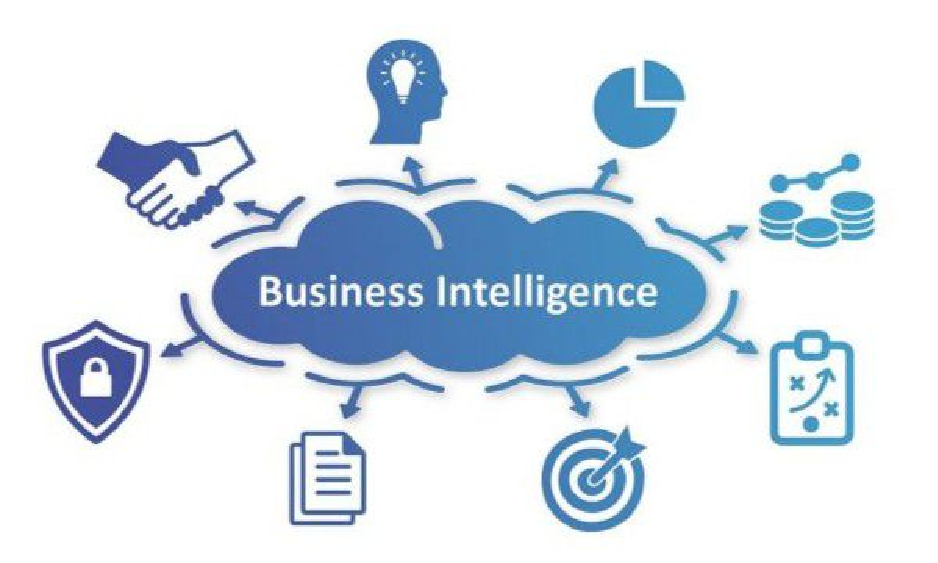
\includegraphics[width=0.75\linewidth]{figure//capitolo_3/Business Intelligence.pdf}
    \caption{La Business Intelligence}
    \label{fig:Business Intelligence}
\end{figure}

Come abbiamo potuto vedere in precedenza, per i processi di analisi e gestione dei dati non esistono delle definizioni fisse che indichino quali processi, protocolli, modelli o infrastrutture siano necessari per poterli svolgere. In un mondo in cui la tecnologia è in continua evoluzione, tali elementi cambiano con essa, differenziando inoltre da azienda ad azienda e da business a business a seconda delle situazioni e necessità. Per questo motivo si può generalizzare il concetto dicendo che «la business intelligence è essenzialmente una conoscenza del business tempestiva, accurata, di alto valore e perseguibile, nonché i processi di lavoro e le tecnologie utilizzate per ottenerla» \cite{bi_for_dummies}.

Quindi, la BI è identificabile come il risultato finale e naturale dell'unione di diversi sistemi e processi, definiti precedentemente, atti a supportare il processo decisionale di un'azienda. L'emergere dell'uso di sistemi di data warehousing, i progressi svolti nella pulizia dei dati, le maggiori capacità di hardware e software e l'evoluzione delle tecnologie connesse ad Internet si combinano per creare un ambiente ricco ed utile per la business intelligence. Principalmente, la BI attinge informazioni da differenti sistemi, riassunti visivamente nella figura \ref{fig:Business Intelligence Systems} \cite{researchgate_bi_systems}.

\begin{figure}[!h]
    \centering
    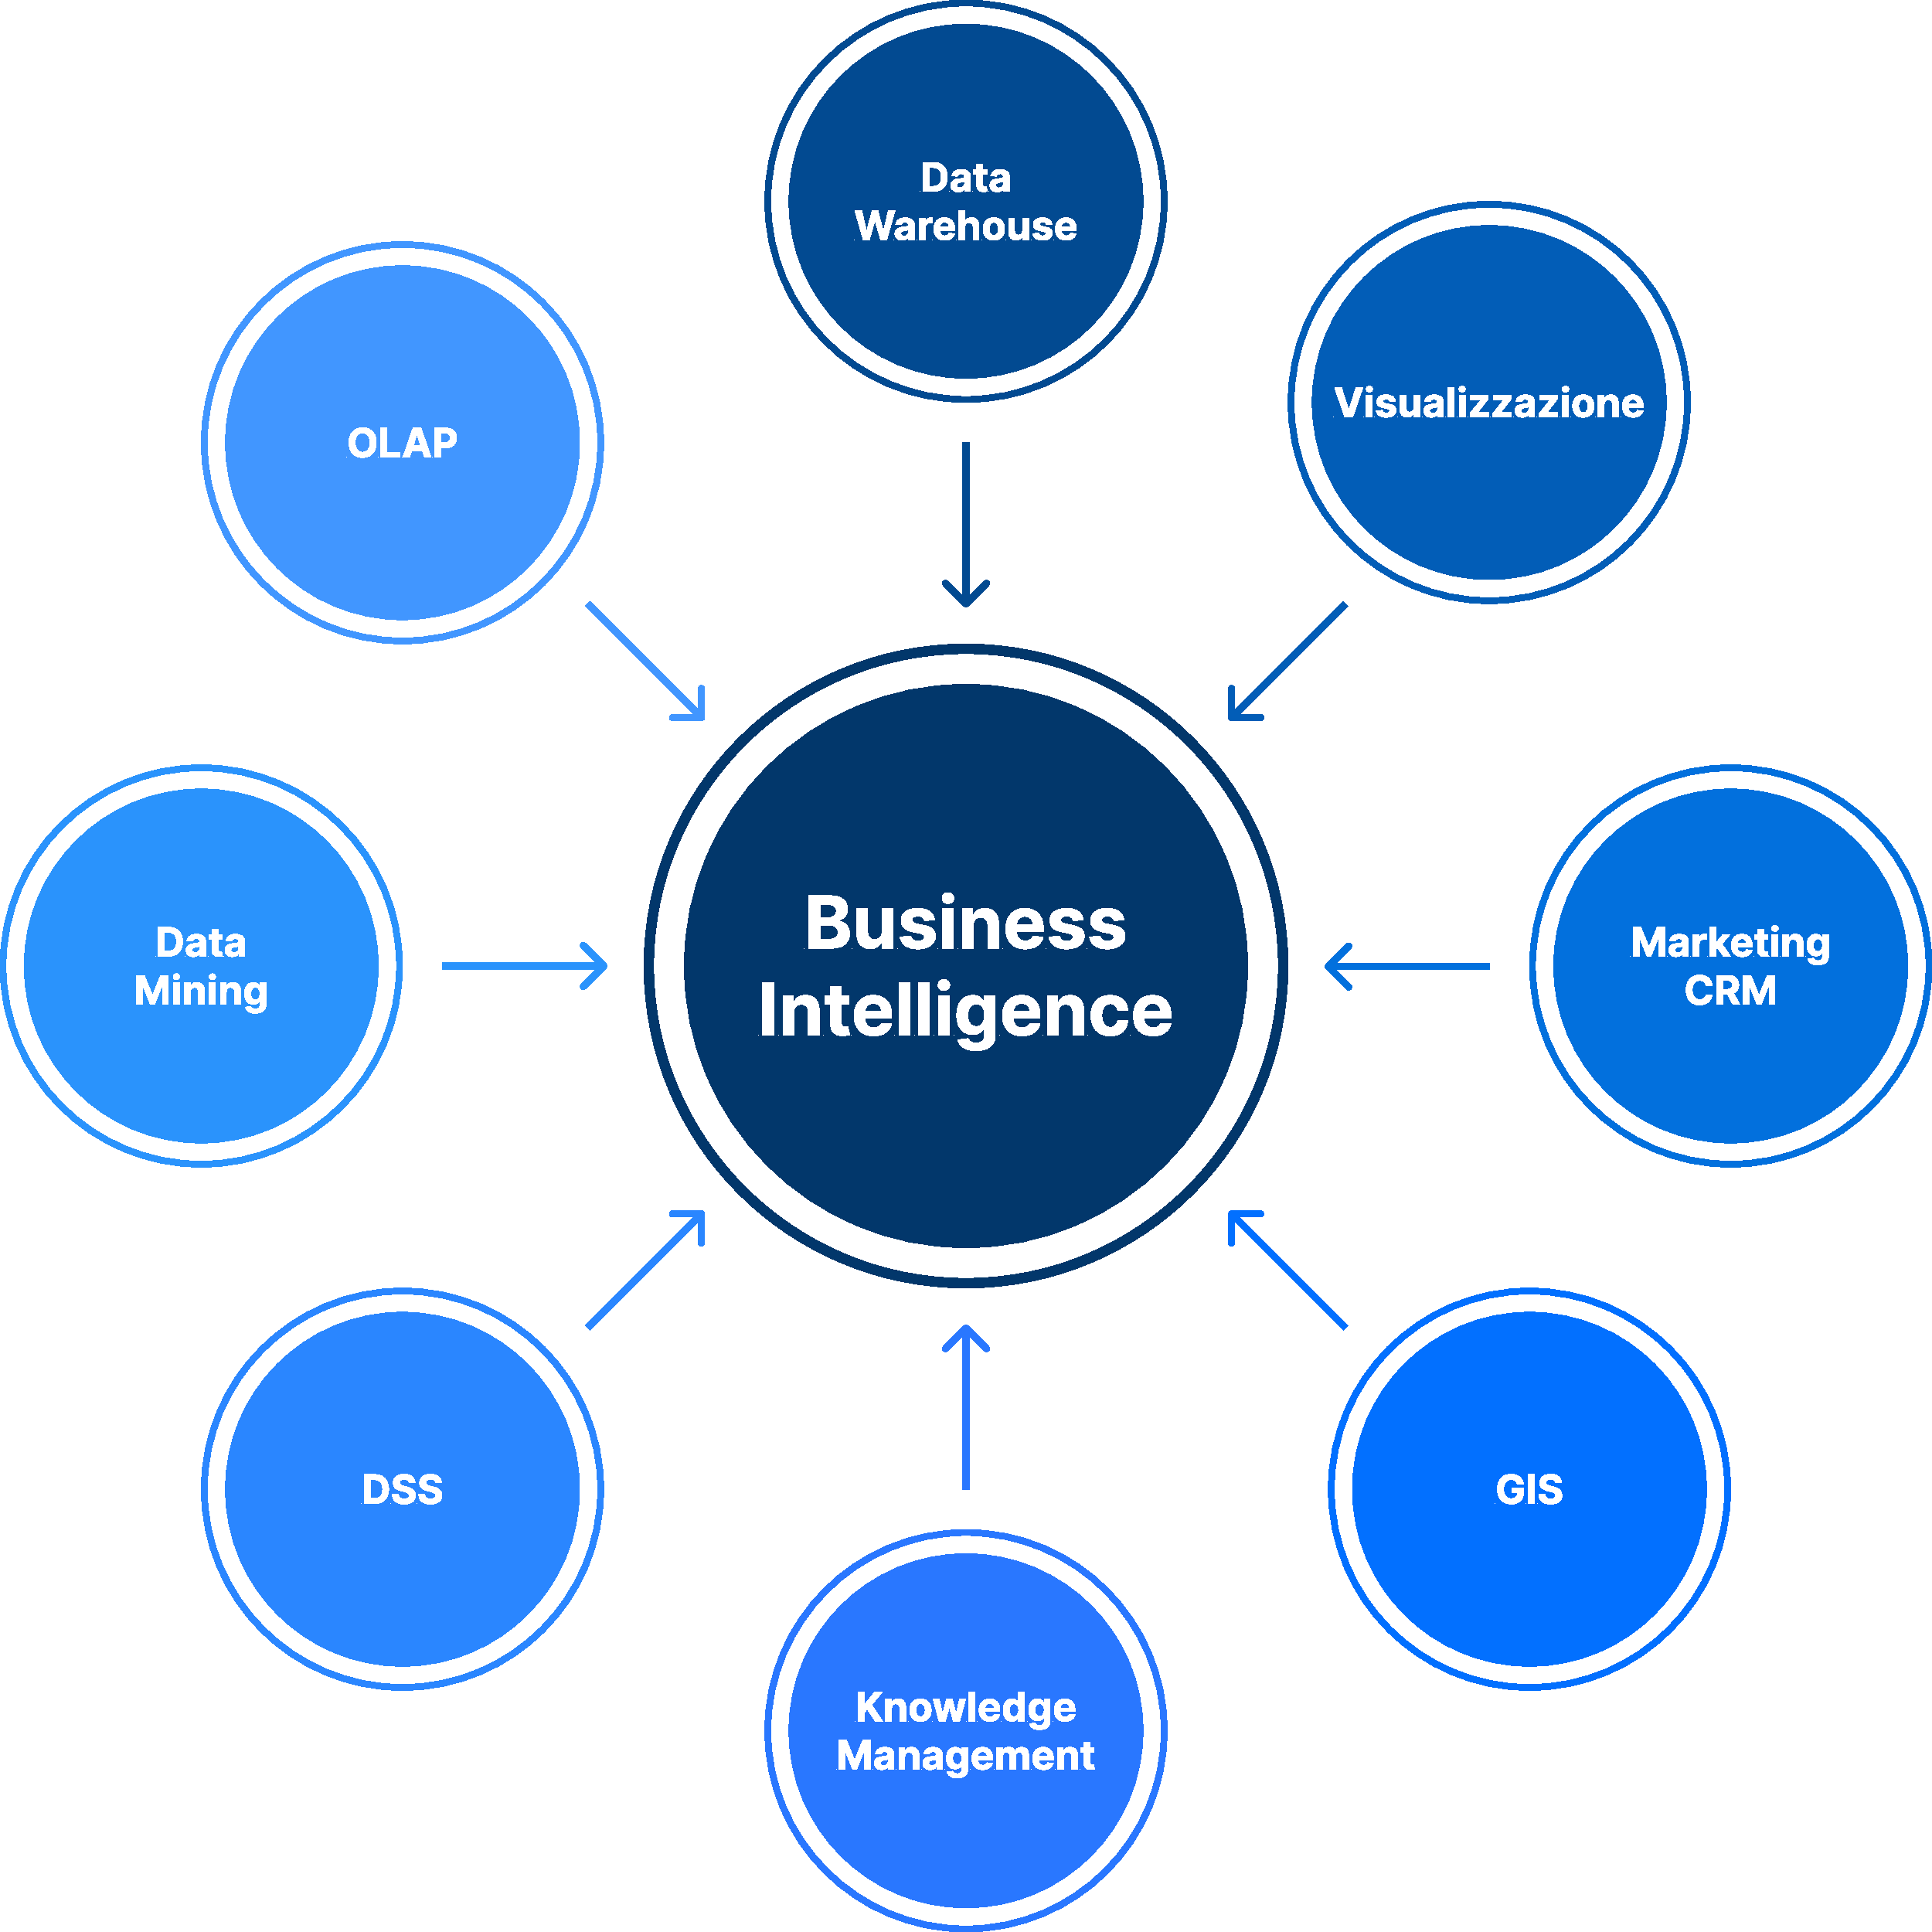
\includegraphics[width=1\linewidth]{figure//capitolo_3/Business Intelligence Systems.pdf}
    \caption{Sistemi di integrazione con la Business Intelligence}
    \label{fig:Business Intelligence Systems}
\end{figure}

\subsection{L'Apporto della Business Intelligence}

L'apporto della business intelligence all'interno di un'azienda è identificabile sotto diversi punti di vista, approfonditi nei paragrafi seguenti.

\subsubsection{Il Valore}

Dal punto di vista economico, il valore aziendale di un investimento è misurato come il \textit{valore attuale netto dei flussi di cassa} (\textit{CFAT})\footnote{\textit{Il flusso di cassa al netto delle tasse} è una misura della performance finanziaria che mostra la capacità di un'azienda di generare flussi di cassa (ovvero, la liquidità netta e gli equivalenti liquidi trasferiti dentro e fuori da un'azienda) attraverso le sue operazioni \cite{cfat_definition}.} dopo le imposte associate all'investimento in questione.
Allo stesso modo, un investimento nell'abito della Business Intelligence crea un bene che deve essere adoperato per generare CFAT incrementali, per far si che comporti aumento delle entrate, riduzione dei costi o entrambi. In altre parole, il valore aziendale della BI risiede nel suo utilizzo all'interno dei processi di gestione, influenzando così i processi operativi che generano entrate o riducono costi, e/o nel suo utilizzo all'interno degli stessi processi operativi che lo adottano \cite{decisionpath_bi_value}.

\subsubsection{I Benefici}

Nella gestione aziendale un efficiente accesso ai dati può costituire uno strumento di business in grado di migliorare l'efficacia dei processi decisionali, grazie soprattutto alla individuazione delle informazioni necessarie a perseguire uno dei principi che costituiscono il punto di forza per eccellenza, ovvero il miglioramento continuo. Nell'ottica di un costante processo di miglioramento può essere determinante l'individuazione dei possibili punti di forza e/o di debolezza del core business, oltre all'individuazione delle opportunità e delle vulnerabilità, definendo le linee guida e le istruzioni operative che solo da una analisi approfondita possono scaturire, grazie anche ad un approccio derivante da una pianificazione strategica aziendale consapevole \cite{dalla_bi_al_dw}.

Per questo motivo, le aziende hanno iniziato ad adoperare sistemi di Business Intelligence nei propri processi decisionali. Per comprendere meglio a cosa sia dovuto questo alto valore di \textit{ROI}\footnote{Il \textit{Return Of Investment} (\textit{ROI}, o \textit{ritorno sull'investimento}) è una misura di performance utilizzata per valutare l'efficienza o la redditività di un investimento misurando direttamente l'ammontare del rendimento di un particolare investimento rispetto al suo costo \cite{investopedia_roi}.} di seguito sono riportati tutti i vantaggi ricavabili dall'uso della BI nella propria azienda \cite{oracle_business_intelligence}.

\begin{itemize}
    \item Migliorare l'accuratezza dei dati.
    \item Prendere decisioni migliori più rapidamente.
    \item Migliorare i risultati mission-critical.
    \item Condividere i dati tra aree funzionali della stessa azienda.
    \item Ottenere una maggiore visibilità delle informazioni finanziarie e operative.
    \item Identificare e ridurre le inefficienze.
    \item Eliminare sprechi, frodi e abusi.
    \item Migliora la produttività e il morale dei lavoratori.
    \item Aumentare il ritorno sull'investimento riducendo il costo totale di proprietà.
    \item Migliorare la trasparenza e il servizio a tutti i livelli.
\end{itemize}

\subsubsection{I Punti Chiave che Indicano la Necessità di BI}

Di seguito sono riportati otto punti chiave che indicano la necessità da parte di un'azienda dell'adozione di una soluzione di Business Intellingence per migliorare la propria gestione \cite{boomper_book_of_bi}.

\begin{itemize}
    \item \textit{Difficoltà nell'accesso ai dati}. In settori competitivi, è essenziale che le aziende possano accedere rapidamente ai propri dati. Di conseguenza, è essenziale che i decision maker accedano a specifiche informazioni con facilità e immediatezza.
    \item \textit{Dati provenienti da diverse fonti}. Quando un'azienda raccoglie dati da varie fonti, consolidarli in informazioni utili può essere difficile (diversi dipartimenti possono adottare metodologie o formati differenti per il salvataggio e il reporting dei dati). La BI può contribuire a unificare questi dati.
    \item \textit{Dipendenza dai fogli di calcolo}. Utilizzare i fogli di calcolo come principale mezzo per archiviare le informazioni con l'aumentare dei volumi di dati e della loro complessità è un processo inefficiente, tedioso e complicato. Una soluzione di BI può contribuire a razionalizzare il processo di raccolta, analisi e reportistica.
    \item \textit{Blocchi nella reportistica}. In molte aziende, la business intelligence e la reportistica sono completamente di competenza del reparto \textit{IT}\footnote{Il termine \textit{IT} fa riferimento all'intero spettro di tecnologie per l'elaborazione delle informazioni (compresi software, hardware, tecnologie di comunicazione e servizi correlati). Generalmente, l'ambito dell'IT non include tecnologie integrate che non generano dati per uso aziendale\cite{gartner_it}.}. Ciò può creare blocchi nel processo di reportistica e ritardi che possono rendere obsolete le informazioni. Una soluzione di BI può contribuire a ridurre questi blocchi dando più potere alle persone attraverso la capacità di autogestire e creare i propri report senza la necessità di conoscenze o esperienza tecniche.
    \item \textit{I tuoi dati non forniscono insight attuabili}. Le aziende possono spesso focalizzarsi così tanto sul processo di raccolta dati che finiscono col trascurare l'importanza della produzione di \textit{insight}\footnote{Le \textit{insight}, o \textit{intuizioni}, sui dati sono le conoscenze che un'azienda ottiene analizzando insiemi di informazioni relative a un determinato argomento o situazione, fornendo in questo modo spunti che aiutano le aziende a prendere decisioni \cite{datarobot_insight}.} applicabili. Per questo motivo le aziende dovrebbero adottare un approccio basato sulla qualità piuttosto che sulla quantità dei dati (evitando di raccogliere semplicemente grandi quantità di informazioni prive di significato).
    \item \textit{Dati obsoleti}. Uno dei principali problemi che affligge le aziende è che i loro dati non sono aggiornati. Ciò potrebbe dipendere da ritardi nella raccolta, analisi o reportistica delle informazioni e può avere conseguenze negative sulle prestazioni aziendali. Una soluzione di BI può automatizzare l'elaborazione e la consegna dei dati, con molte soluzioni in grado di pianificare i report in anticipo, garantendo che i dirigenti aziendali dispongano sempre delle informazioni necessarie.
    \item \textit{Difficoltà nella visualizzazione dei dati}. La visualizzazione dei dati è una parte fondamentale dell'analisi dati, ma senza l'esistenza di una soluzione di BI, spesso viene trascurata. I dati una volta raccolti andrebbero sfruttati per essere definibili come utili.
    \item \textit{Impossibilità di accedere ai dati su dispositivi multipli}. Al giorno d'oggi, è sempre più importante che le informazioni siano accessibili in qualunque momento e luogo. Per questo motivo nuovi strumenti di BI sono indirizzati verso un approccio che permetta di utilizzarli da dispositivi multipli.
\end{itemize}

\subsection{Sviluppo di Una Soluzione Aziendale}

\subsubsection{Processo Ciclico}
Un processo di Business Intelligence, per quanto possa differire per approccio, l'argomento e lo scopo di riferimento, in generale è caratterizzato da alcuni passaggi fondamentali per la sua implementazione, ovvero \cite{citeseerx_bi_process}:

\begin{enumerate}
    \item \textit{Analisi}. Prima di essere predisposto per l'utilizzo, è necessario svolgere un'analisi dei requisiti che indichi quali sono i \textit{KPI}\footnote{Un \textit{indicatore chiave di prestazioni} (\textit{Key Performance Indicator}, o \textit{KPI}) si riferisce ad una misurazione quantificabile utilizzata per valutare le prestazioni a lungo termine di un'azienda rispetto a quello specifico ambito di interesse, aiutando a determinare i risultati strategici, finanziari e operativi di una compagnia (potendo anche metterli a paragone con altri competitor dello stesso settore)\cite{investopedia_kpi}.} richiesti dagli utenti finali. Tale fase permette di identificare, ad alto livello, i vari componenti che una possibile soluzione dovrebbe integrare.
    \item \textit{Progettazione}. Sulla base dei requisiti stilati nella fase precedente, in questa vengono identificate specificatamente quali tecnologie siano appropriate per rendere reale la soluzione precedentemente ideata.
    \item \textit{Sviluppo}. Questa fase comporta la messa in atto di tutti i processi studiati, delle infrastrutture progettate e dei modelli di analisi scelti. L'implementazione, inoltre, dipende spesso anche dalla tipologia di dati che dovranno essere gestiti dal sistema, poiché ognuno può necessitare di funzionalità differenti.
    \item \textit{Distribuzione}. Una volta implementata e testata, la soluzione viene messa a disposizione degli utenti finali. Sono proprio quest'ultimi le persone da cui dipende la riuscita finale del progetto, poiché tale fase include lo sviluppo di report e analisi predefinite per i decision maker aziendali.
    \item \textit{Evoluzione}. Tale fase si può dire che è ciò che rende ciclico l'intero processo appena esplicato. Questo perché bisogna sempre valutare il successo del sistema creato per poi estenderlo con ulteriori funzionalità e anche modificare, ottimizzare e rivalutare scelte fatte in precedenza.
\end{enumerate}

\begin{figure} [H]
    \centering
    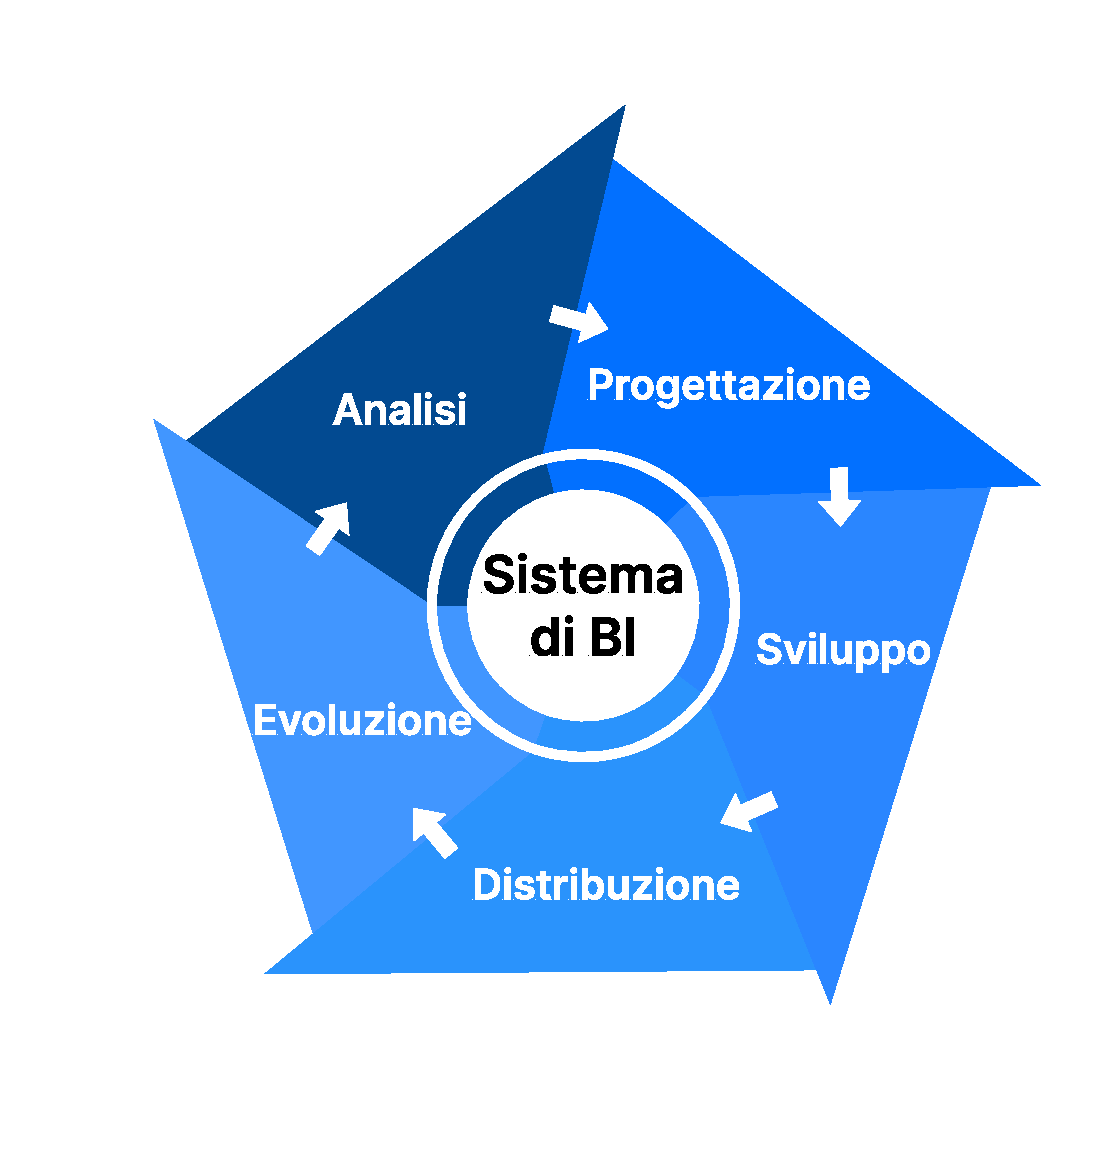
\includegraphics[width=0.75\linewidth]{figure//capitolo_3/Business Intelligence Life Cycle.pdf}
    \caption{Ciclo di vita di un processo di Business Intelligence}
    \label{fig:Business Intelligence Life Cycle}
\end{figure}

\subsubsection{Modello Approfondito}

In modo più approfondito, l'implementazione di un sistema di Business Intelligence si compone di 8 fasi differenti \cite{altexsoft_bi_implementation}:

\begin{enumerate}
    \item \textit{Introduzione della BI ai dipendenti e agli stackholder}. Per poter sfruttare a pieno un sistema di BI è necessario far apprendere a tutti gli stakeholder\footnote{Uno \textit{stakeholder} è una parte (individuo, gruppo o organizzazione) che ha interesse in un'azienda e può influenzare o essere influenzata dalle sue attività (ad esempio, investitori, dipendenti, clienti o fornitori) \cite{investopedia_stakeholder}}. Le sue possibili funzionalità ed obiettivi. A seguito di una prima spiegazione, è poi necessario identificare il problema che si vuole risolvere o analizzare.
    \item \textit{Definizione di obiettivi, KPI e requisiti}. Una volta identificato il problema che si vuole affrontare, è necessario definire quali sono gli obiettivi che si vogliono raggiungere e quali possono essere (ipoteticamente parlando) dei KPI e metriche di valutazione rilevanti nell'ambito di interesse (possono essere sia vincoli finanziari che indici di prestazione). Ciò permetterà di comprendere anche quali sono i requisiti necessari allo sviluppo ed utilizzo della soluzione ricercata.
    \item \textit{Scelta degli strumenti o di una soluzione personalizzata}. A seguito della definizione dei requisiti è possibile comprendere quale soluzione possa essere la migliore da adoperare nel proprio sistema. Esistono molte soluzioni, tuttavia una soluzione personalizzata ad hoc per un'azienda può essere la scelta più adatta. Per comprendere quale sia la soluzione più conveniente è necessario svolgere una ricerca di mercato che permetta di mettere a paragone tutte le possibili scelte.
    \item \textit{Definizione di un team predisposto}. Per poter sfruttare al meglio un sistema del genere spesso è necessario definire un team predisposto a tale compito. Solitamente si cerca di inserire nel team persone di differenti reparti in modo da avere un possibile contatto diretto con gli stessi e personale conoscente del proprio ambito di lavoro. Inoltre, l'eterogeneità del gruppo permetterà una possibile evoluzione dello stesso grazie a punti di vista e pensieri differenti.
    \item \textit{Documentazione della strategia adottata}. Per creare un sistema nel modo corretto e senza errori, all'interno del progetto in questione viene adottata una specifica strategia. Tale strategia può includere differenti componenti, per questo motivo è importante riportare una documentazione che spieghi per ognuno di essi l'approccio adottato a riguardo.
    \item \textit{Configurazione di strumenti di integrazione e data warehouse e scelta di un approccio architetturale}. Tale fase dipende molto dallo strumento adottato, una scelta personalizzata o una \textit{plug and play} avranno impatti differenti sulla difficoltà e capacità di integrazione con le infrastrutture e software dell'azienda.
    \item \textit{Implementazione di un'interfaccia utente finale}. In questa fase i dati vengono modellati, gestiti e infine messi a disposizione degli utenti finali grazie ad un'apposita interfaccia degli strumenti di BI. La creazione di corretti report è una fase essenziale e critica perché permette l'analisi e la comprensione delle informazioni necessarie a prendere decisioni basate su tutti i dati gestiti dal sistema.
    \item \textit{Formazione degli utenti finali}. Un'ulteriore fase che può essere affrontata è la formazione degli utenti finali in modo da agevolare l'interazione e integrazione degli strumenti nei normali processi di gestione e sviluppo del personale aziendale. In caso contrario, si potrebbe riscontrare un problema di un utilizzo scorretto o sbagliato da parte degli utenti dello strumento messo a disposizione.
\end{enumerate}

\begin{figure} [H]
    \centering
    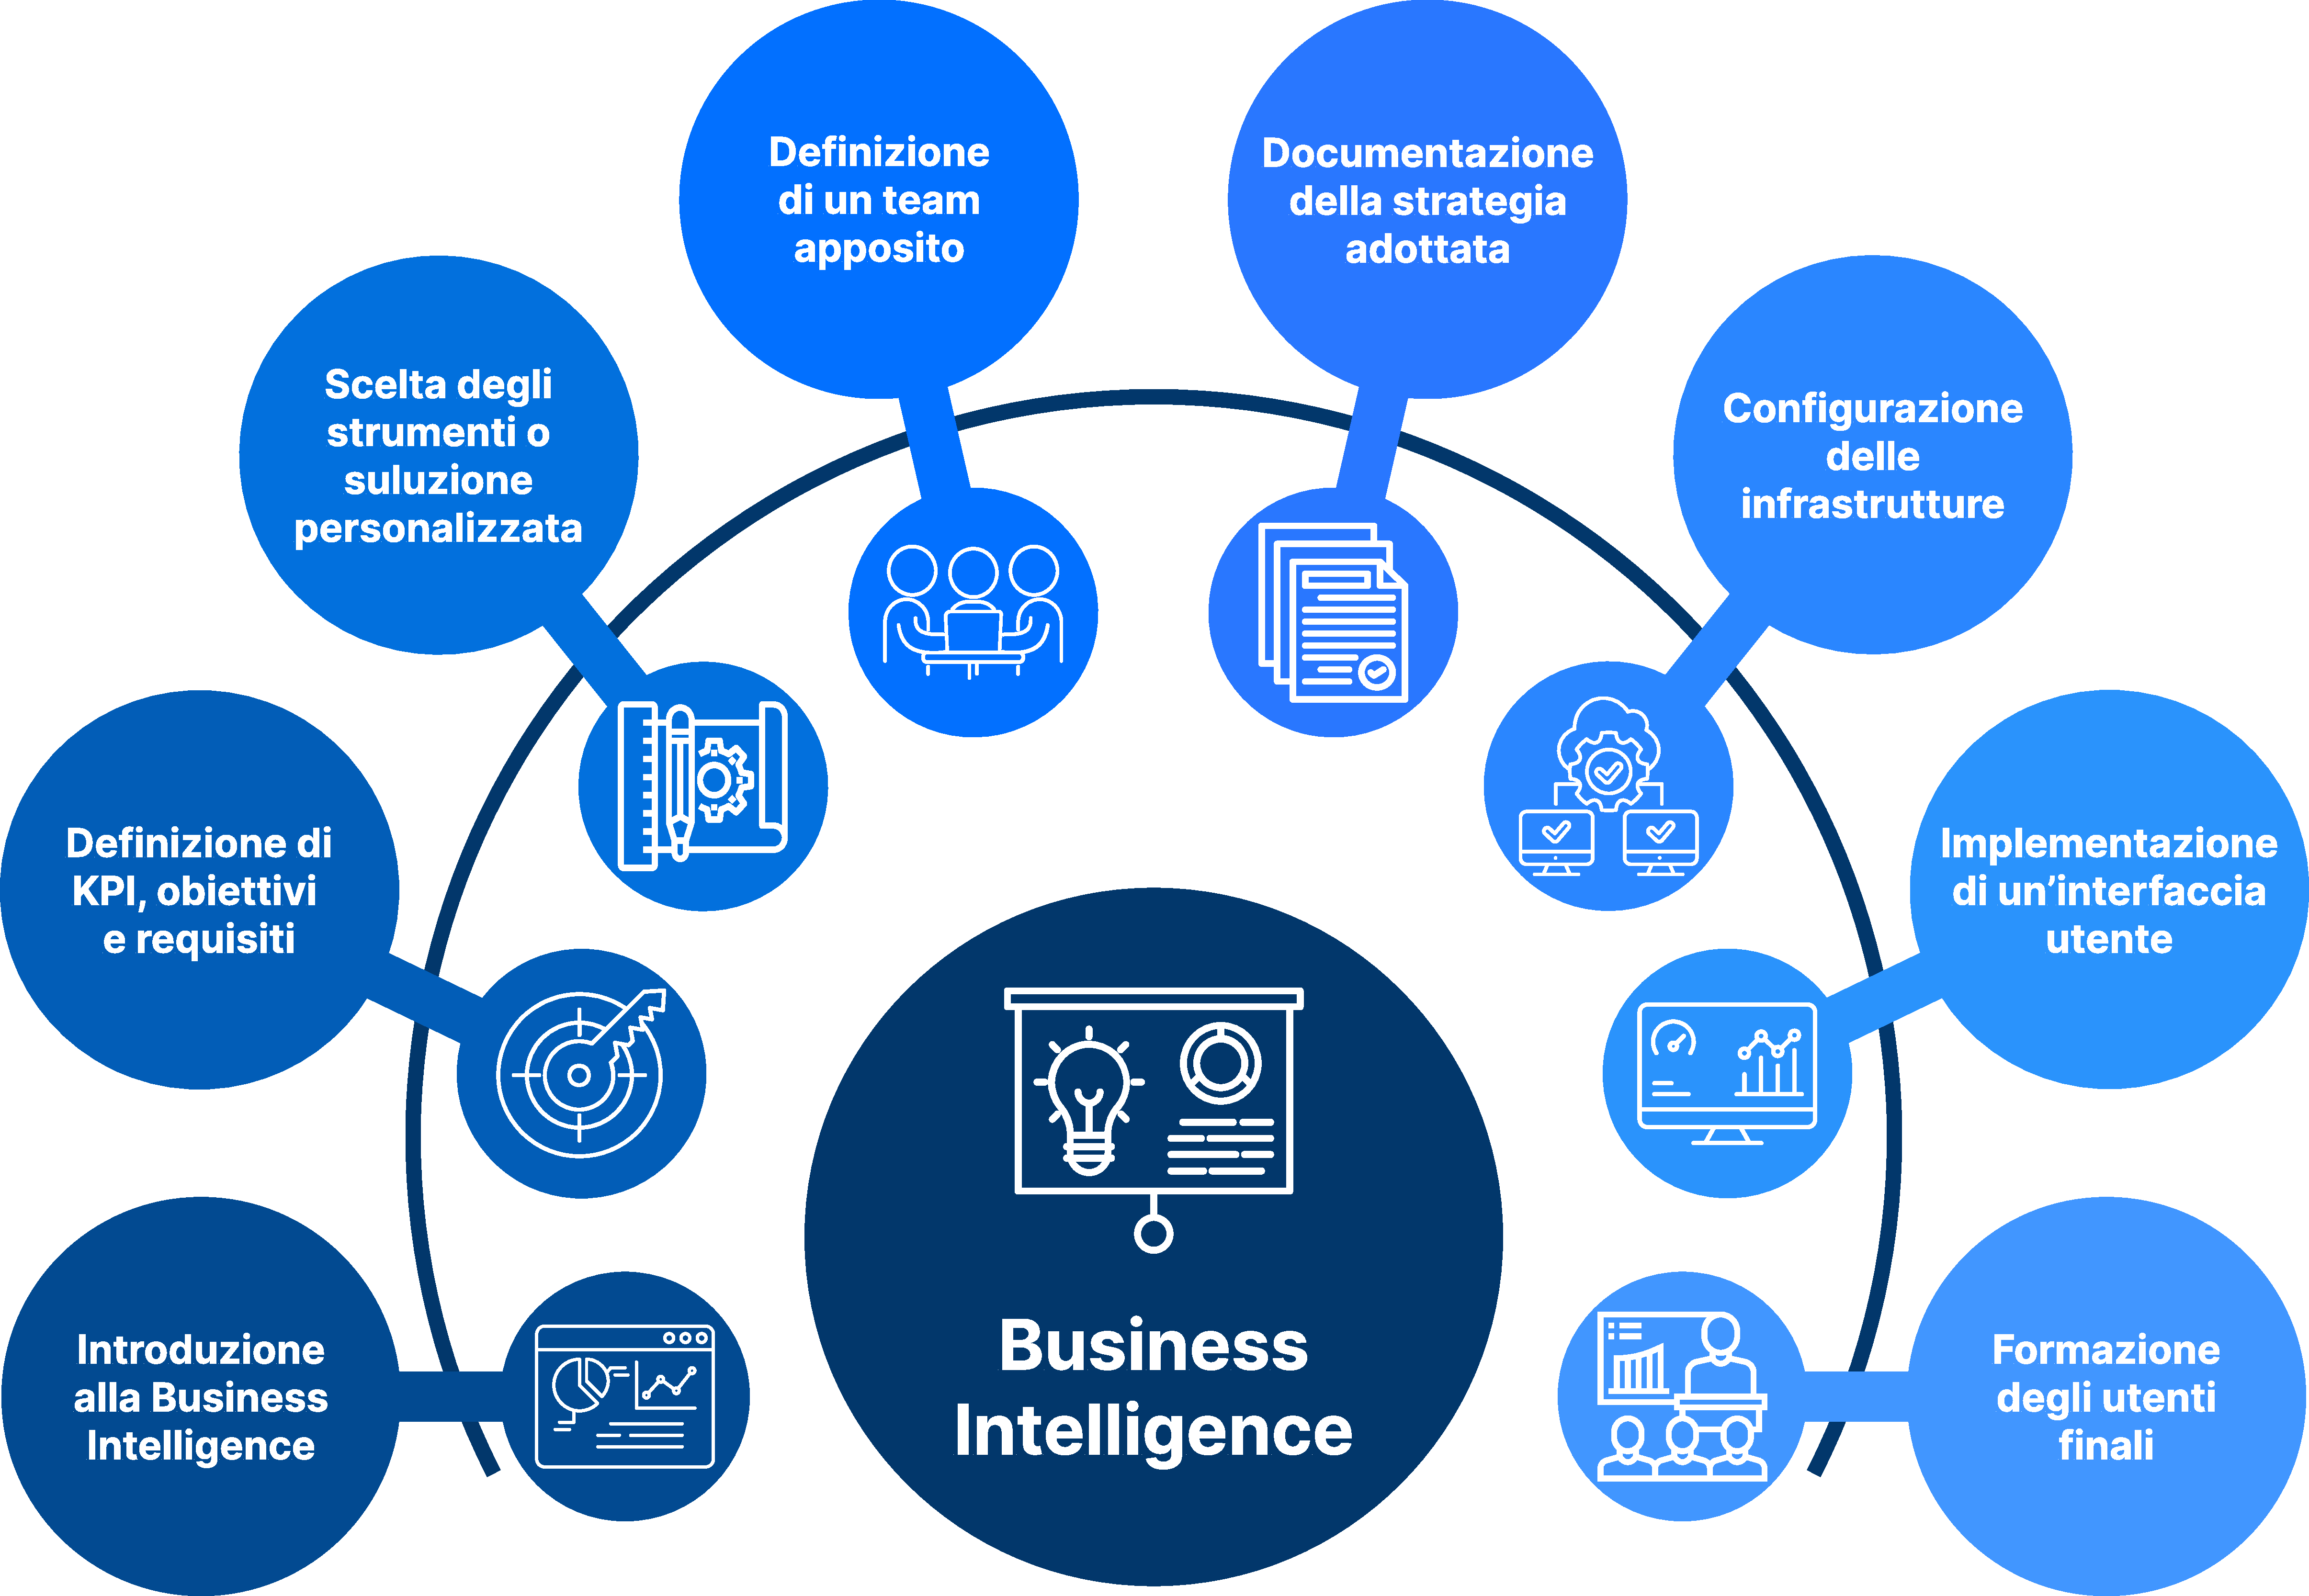
\includegraphics[width=1\linewidth]{figure//capitolo_3/Business Intelligence Process.pdf}
    \caption{Processo di adozione di un sistema di Business Intelligence}
    \label{fig:enter-labelBusiness Intelligence Process}
\end{figure}

\subsection{Le Capacità della BI}

Le capacità della Business Intelligence sono competenze fondamentali che aiutano le aziende a migliorare la propria attitudine all'adattamento al cambiamento e all'esecuzione. Per quanto siano molte le ricerche a riguardo, è rimasto in gran parte silente il ruolo delle capacità della BI nel raggiungere l'adeguato abbinamento tra la BI e l'ambiente decisionale in cui è implementata. Di seguito sono riportate le capacità precedentemente accennate \cite{bi_capabilities}:

\begin{itemize}
    \item \textit{Qualità dei dati}. La BI si basa principalmente sui dati numerici, che vengono analizzati, gestiti e misurati. Proprio per questo motivo la qualità dei dati è un requisito fondamentale ed imprescindibile in questo mondo. Quando si parla di qualità dei dati si intende che essi siano consistenti e completi, perché diversamente non avrebbero una grossa affidabilità.
    \item \textit{Integrazione con altri sistemi}. Poiché il sistema di BI dipende da altri sistemi, un'importante caratteristica è la sua capacità di interoperabilità con questi. In questo caso, quando si parla di integrazione, si intende sia in ambito software che in ambito hardware.
    \item \textit{Accesso per gli utenti}. Dato che i sistemi di BI non hanno un solo utilizzo o scopo, non è possibile creare una soluzione onnicomprensiva adattabile a tutti i problemi. Per questo motivo è congeniale mettere a disposizione di utenti diversi gli strumenti di BI, in modo che questi possano creare i propri report e svolgere le relative analisi in totale autonomia senza alcuna difficoltà.
    \item \textit{Flessibilità}. Per far sì che una soluzione sia ottimale, è necessario che questa si adatti alle necessità e all'evoluzione dei dati e dell'organizzazione stessa (tecnologie e normative da dover applicare).
    \item \textit{Supporto alla gestione del rischio}. La gestione del rischio permette di aiutare nella presa di decisioni in condizioni spesso incerte. Questa capacità è cruciale per le organizzazioni che operano in ambienti ad alto rischio. Poiché nonostante esistano rischi e instabilità in ogni decisione aziendale, le compagnie cercano di adottare sistemi che possano diminuire tale rischio, e la BI è uno di questi.
\end{itemize}

\subsection{Business Process intelligence (BPI)}

La progettazione dei processi e le tecnologie di automazione vengono sempre più utilizzate dalle aziende che cercano di migliorare le qualità e l'efficienza dei loro processi amministrativi e produttivi e fornire rapidamente e in modo affidabile servizi alle aziende e ai clienti individuali. Per svolgere queste attività al meglio, sono molte le aziende che decidono di adottare delle soluzioni che prendono il nome di \textbf{Business Process intelligence} (\textit{BPI}). Con questo termine si fa riferimento all'applicazione di tecniche di BI per lo sviluppo e l'implementazione di processi aziendali e comprende molte ambiti di applicazione (ad esempio, monitoraggio, analisi e scoperta dei processi, controllo di conformità, operazioni di previsione ed ottimizzazione), ovvero nell'ambito della \textit{BPM}\footnote{Il \textit{Business Process Management} (\textit{BPM}) è una disciplina che adotta diversi metodi per scoprire, modellare, analizzare, misurare, migliorare e ottimizzare i processi aziendali \cite{gartner_bpm}.} \cite{academiaedu_bpi_definition}.

\begin{figure}[H]
    \centering
    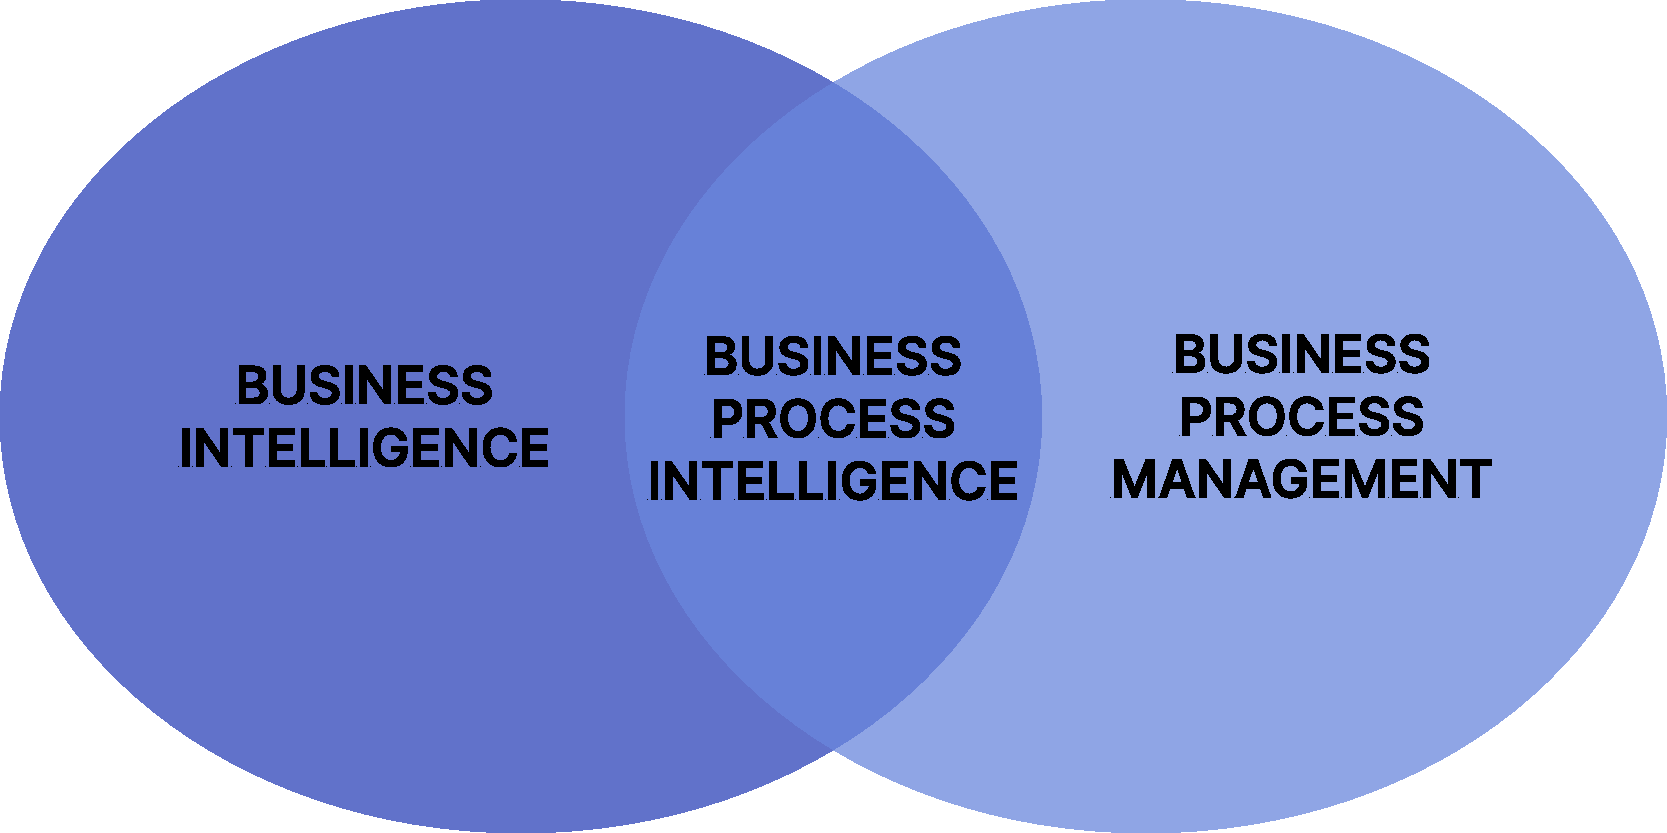
\includegraphics[width=0.75\linewidth]{figure//capitolo_3/Business Process Intelligence.pdf}
    \caption{La Business Process Intelligence}
    \label{fig:Business Process Intelligence}
\end{figure}

Date le molteplici possibilità e l'elevato spettro di applicazione, la business process intelligence dispone di diverse funzionalità che offrono altrettanti livelli di automazione per la gestione della qualità dei processi, ovvero \cite{academiaedu_bpi_feautures}:

\begin{itemize}
    \item \textit{Analisi}. La BPI permette agli utenti di analizzare le esecuzioni dei processi completati sia dal punto di vista aziendale che da quello programmatico per gli operatori IT. Inoltre, non solo offre molti sistemi di reportistica, ma la BPI permette anche di analizzare la progettazione di un modello di processo e identificare le tecniche per poterlo migliorare.
    \item \textit{Predizione}. La BPI permette di applicare modelli predittivi ai processi in esecuzione in modo da poter identificare preventivamente la possibilità di riscontrare eccezioni o comportamenti imprevisti e indesiderati. Anche in questo caso, è possibile avere un punto di vista aziendale oppure programmatico.
    \item \textit{Monitoraggio}. La BPI può monitorare ed analizzare le istanze dei processi che sono in esecuzione e informare l'utente nel caso vengano riscontrate situazioni insolite. Grazie a ciò, un utente può visualizzare e analizzare lo stato attuale del sistema, dei processi, dei servizi e delle risorse attualmente in uso e attività. Inoltre, con determinati principi di automazione, è possibile svolgere azioni predefinite in caso di situazioni critiche.
    \item \textit{Controllo}. La BPI, sfruttando il monitoraggio e la predizione dei processi, può interagire con il \textit{BPMS} (\textit{Business Process Management System}) per evitare delle degradazioni di qualità previste ed effettive.
    \item \textit{Ottimizzazione}. La BPI può individuare delle possibili aree di miglioramento nelle definizioni dei processi aziendali attualmente in uso e nell'assegnazione delle risorse ai relativi servizi in attività. Ciò permette una possibile diminuzione dei costi e un aumento dell'efficienza dei processi.
\end{itemize}

\subsection{La Business Analytics}

Oltre alla Business Intelligence, per quanto meno conosciuta, esiste anche la \textbf{Business Analytics} (\textbf{BA}) che comprende soluzioni adottate per definire modelli di analisi e simulazioni per creare scenari, comprendere la realtà e prevedere possibili future situazioni. La BA include strumenti di data mining, analisi predittiva, analisi approfondita e statistica per essere fornita come un sistema di utilità per un'utente aziendale \cite{gartner_ba}.

A primo impatto la Business Analytics può sembrare identica alla Business Intelligence, ed effettivamente sono molto simili tra loro, tuttavia esiste una differenza minima quanto sostanziale, ovvero l'adozione dell'analisi predittiva con l'obiettivo di comprendere possibili eventi futuri. In altre parole, sia la BI che la BA sfruttano i dati di eventi e azioni passate ma lo fanno con scopi differenti: la prima focalizza il proprio obiettivo sul comprendere cosa sia accaduto in passato, mentre la seconda focalizza il proprio obiettivo sul comprendere come agire in futuro \cite{talend_bi_vs_ba}.


\subsubsection{Differenze tra BI e BA}
Per essere più precisi, è possibile affermare che la Business Intelligence adotta l'\textbf{analisi retrospettiva} (\textit{analisi diagnostica} e \textit{analisi descrittiva}), mentre la Business Analytics adotta l'\textbf{analisi prospettiva} (\textit{analisi prescrittiva} e \textit{analisi predittiva}) \cite{researchgate_bi_and_ba_analytics}.

Per comprendere meglio le differenze tra le due tipologie di analisi, di seguito è riportata una tabella riepilogativa \cite{knowledgehut_bi_vs_ba}:

\begin{comment}
\begin{table}
    \centering
    \begin{tabular}{ccc}
        Parametri & Business Intelligence & Business Analytics\\
        Definizione & 
        La BI riguarda la comprensione del passato e del presente di un'azienda.& La BA riguarda la previsione dei risultati futuri delle azioni intraprese dall'azienda.\\
        Focus & 
        Gli strumenti di BI si concentrano sulla gestione dei dati.& 
        Gli strumenti di BA si concentrano sull'analisi dei dati.\\
        Applicazioni & 
        Gli strumenti di BI sono progettati per fornire informazioni dettagliate sulle prestazioni della tua azienda nel tempo.&
        Gli strumenti di BA sono progettati per aiutare a prendere decisioni migliori su come ottimizzare le operazioni per il futuro.\\
        Approccio & 
        La BI si concentra sull'analisi diagnostica e sull'analisi descrittiva.& 
        La BA si concentra sull'analisi predittiva e sull'analisi prescrittiva.\\
        Utilizzo & 
        La BI si concentra in genere sul reporting a livello aziendale tra più dipartimenti e team.& 
        La BA in genere si concentra sull'analisi dettagliata di aree specifiche all'interno di un'organizzazione (ad esempio come il marketing).\\
    \end{tabular}
    \caption{Differenze tra Business Intelligence e Business Analytics}
    \label{tab:BI vs BA}
\end{table}
\end{comment}

%TODO: Controllare se va aggiunta qualche introduzione o prologo di collegamento

\section{La Conoscenza}

Per anni gli esseri umani hanno discusso sul significato di “\textit{conoscenza}”, su cosa significhi conoscere qualcosa e su come le persone possano generare e condividere nuova conoscenza. Nonostante l'importanza di tale dilemma nelle discussioni affrontate nel corso della storia, solo negli ultimi anni il mondo del business ha iniziato a riconoscere l'importanza della conoscenza come una risorsa \cite{knowledge_management_tools}.
La crescente evoluzione del mondo del Data Warehousing e dei Big Data ha portato alla necessità di svolgere studi, generare teorie o modelli e progettare strumenti che potessero aiutare le persone nell'estrazione di informazioni, ritenute, utili. Questa branca del mondo digitale prende il nome di \textbf{Knowledge Discovery in Databases} (\textit{KDD}), ovvero \textit{scoperta della conoscenza dei database}.

\subsection{La Piramide della Conoscenza}
Finora abbiamo parlato del mondo dell'analisi dei dati dando per scontato il concetto del legame tra i dati e la conoscenza, per quanto sia stata puntualizzata più volta la loro rilevanza. «Tipicamente l'informazione è definita in termini di dati, la conoscenza in termini di informazione e la saggezza in termini di conoscenza», queste sono le parole della giornalista Jennifer Rowley \cite{rowley_dikw_hierarchy}, che permettono di descrivere brevemente la rappresentazione della \textit{piramide della conoscenza}, meglio conosciuta come \textbf{DIKW pyramid} (\textit{Data, Information, Kownledge and Windsome pyramid}), ovvero il modello creato per spiegare il processo di trasformazione dei dati e di come essi possano acquistare valore effettivamente, trasformandosi in \textit{informazione}, \textit{conoscenza} e \textit{saggezza}.

\begin{figure}[H]
    \centering
    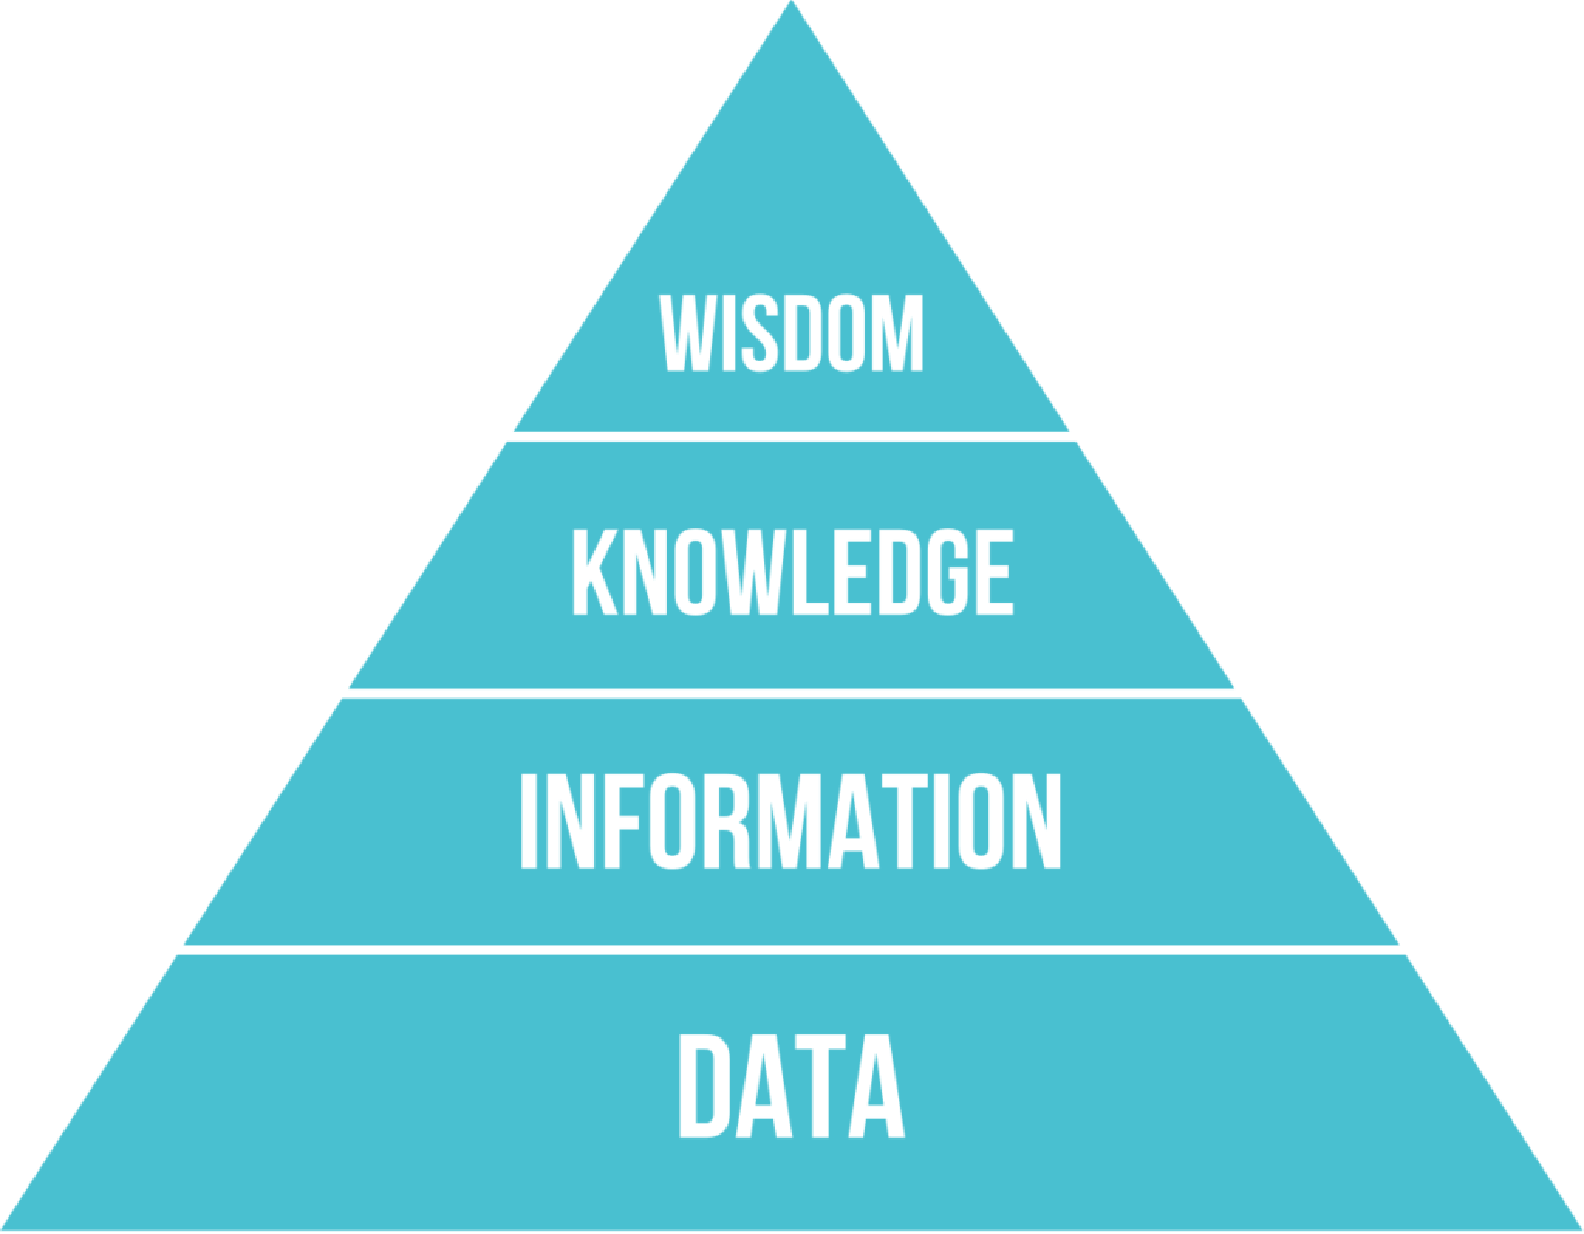
\includegraphics[width=0.6\linewidth]{figure//capitolo_3/DIKW Pyramid.pdf}
    \caption{Piramide della conoscenza}
    \label{fig:DIKW Pyramid}
\end{figure}

L'origine della piramide DIKW è incerta, sia riguardo chi sia il suo creatore che il periodo di creazione, come meglio spiegato dal professor Danny P. Wallace \cite{knowledge_management_historical} «La presentazione delle relazioni tra dati, informazioni, conoscenza e talvolta saggezza in una disposizione gerarchica fa parte del linguaggio della scienza dell'informazione da molti anni. Sebbene non sia chiaro quando e da chi tali relazioni siano state presentate per la prima volta come gerarchia, l'ubiquità della nozione di gerarchia è incorporato nell'uso dell'acronimo DIKW come rappresentazione abbreviata della trasformazione da dati a informazione a conoscenza in saggezza».

Per comprendere meglio tale rappresentazione, è meglio approfondire ognuno dei suoi elementi \cite{researchgate_revising_dikw_pyramid}:
\begin{enumerate}
    \item \textbf{Data} (\textit{Dati}). I dati sono solitamente definiti come fatti e statistiche che vengono ricavati insieme per svolgere riferimenti o analisi. I dati generalmente vengono combinati, ricombinati, confezionati, venduti e ridistribuiti; proprio per questo motivo sono soggetti ad un uso improprio, quasi abuso. Inoltre, bisogna sempre ricordare che la raccolta di dati, anche in ordine di peta, exa o zettabyte, non ha alcun valore se essi possono essere inaccurati, obsoleti oppure intenzionalmente o non falsi. Proprio per questo motivo, i dati non portano sempre delle informazioni direttamente, ed è impossibile concludere che il volume di dati raccolto e archiviato per creare “informazioni” stiano effettivamente creando maggiori o migliori informazioni. È quindi possibile definire che i dati sono fondamentali perché il percorso nella piramide si basa su di loro, tuttavia sono anche definibili inutili poiché da soli non hanno alcun valore.
    \item \textbf{Information} (\textit{Informazione}). Le informazioni, in termini generali, sono comunemente definite come fatti forniti o appresi su qualcosa o qualcuno. Nell'ambito digitale, l'informazione può essere definita come il significato attribuito dagli esseri umani ai dati raccolti o a sottoinsiemi selezionati di dati, tipicamente accompagnato da una presunzione di verità o di fatto. Pertanto, i dati interrogati possono diventare informazioni, ma se l'informazione sia utile o preziosa dipende interamente dal mondo di interrogazione dell'accuratezza dei dati sottostanti. Come espresso in precedenza, le informazioni possono definirsi valide solamente quando la fonte da cui provengono è valida, poiché altrimenti produrranno risultati errati. Ad aumentare l'importanza del valore delle informazioni vi è l'imprescindibile regola per cui per ottenere informazioni valide e utili dai dati è necessario svolgere le domande nel giusto modo e forma. La sbagliata interpretazione delle informazioni è uno scenario molto comune poiché è probabile che accada facilmente. Considerando quanto detto, l'informazione non porta necessariamente alla conoscenza e maggiori informazioni, per quanto corrette, non aumentano sempre la conoscenza. Pertanto, l'informazione potrebbe diventare conoscenza, ma anche essere non utile.
    \item \textbf{Knowledge} (\textit{Conoscenza}). La conoscenza è generalmente definita come fatti, informazioni e competenze apprese attraverso l'esperienza o l'istruzione. Data questa definizione, per quanto corretta, necessita di una precisazione, ovvero è possibile acquisire conoscenza su un argomento attraverso la raccolta di informazioni e le esperienze di vita, ma la conoscenza su un argomento non implica automaticamente la conoscenza su altri argomenti, anche se affini; per questo motivo il processo di acquisizione della conoscenza deve essere ripetuto su ogni argomento. In termini generali, maggiore è la conoscenza di una persona e più è probabile che soddisfi più bisogni umani e che ottenga ulteriore successo nella vita. Conoscenza e saggezza sono strettamente correlate, ma la saggezza comprende sia un volume più ampio che una maggiore durata di conoscenza accumulata.
    \item \textbf{Wisdom} (\textit{Saggezza}). La saggezza è comunemente definita come la qualità di avere esperienza, conoscenza e buon giudizio. A questa definizione si potrebbe aggiungere l'aggettivo “estesa”, poiché quantità limitate di questi elementi non sono sufficienti per creare saggezza. La saggezza si crea attraverso l'informazione, l'esperienza e la conoscenza, oltre all'apporto umano di analisi ed estrapolazione. L'uso intelligente dell'informazione, dell'esperienza e della conoscenza è vitale per la saggezza.
\end{enumerate}

\subsection{Tipologie di conoscenza}

Parlare in termini generici di conoscenza non è sbagliato, tuttavia, sarebbe sicuramente più corretto fare un approfondimento sulle varie categorie in cui la conoscenza può essere suddivisa \cite{getguru_types_of_knowledge}.

\begin{itemize}
    \item \textit{Conoscenza esplicita}. È la conoscenza che riguarda gli argomenti che sono facilmente documentabili in modo sistematico e condivisibili su larga scala.
    \item \textit{Conoscenza implicita}. È la conoscenza acquisita con la messa in pratica. È possibile acquisirla applicando in una situazione specifica la conoscenza esplicita.
    \item \textit{Conoscenza tacita}. È la conoscenza di tipo intangibile che può essere difficile da spiegare in modo diretto. Questo tipo di conoscenza è informale e viene appresa con l’esperienza e solitamente si applica ad una specifica situazione. 
    \item \textit{Conoscenza dichiarativa}. È la conoscenza che si riferisce a informazioni statiche e fatti specifici, di facile accesso, su un determinato argomento. Questa è un tipo di conoscenza in cui l’individuo che la mette in atto è consapevole in modo cosciente della propria comprensione della materia.
    \item \textit{Conoscenza procedurale}. È la conoscenza che si focalizza sul come funzionano determinate cose e viene dimostrata attraverso la capacità di fare qualcosa.
    \item \textit{Conoscenza a posteriori}. È la conoscenza che rappresenta la soggettività acquisita dall'esperienza individuale. Per quanto non debba essere documentata, permette agli individui di avere una presa di coscienza per riconoscere i propri punti di forza e debolezza derivati dalle proprie esperienze passate.
    \item \textit{Conoscenza a priori}. È la conoscenza acquisita indipendentemente dall'esperienza o dalle prove. Questo tipo di conoscenza viene spesso condivisa attraverso il ragionamento logico o la capacità di pensare in modo astratto.
\end{itemize}

\subsection{Gestione della Conoscenza}

La \textbf{gestione della conoscenza} (\textit{GC}, o \textit{Knowledge Management – KM}) aziendale implica la gestione formale delle risorse di conoscenza per facilitarne l'accesso e il riutilizzo, generalmente adoperando tecnologie informatiche avanzate. Il KM viene definito "formale" in quanto la conoscenza viene classificata e categorizzata in base ad un'ontologia\footnote{L'\textit{ontologia} è lo studio dell'essere in quanto tale, nonché delle sue categorie fondamentali \cite{wikipedia_ontologia}.} prestabilita (che però è in continua evoluzione), in dati strutturati e semi-strutturati e in basi (intesi come "insiemi") di conoscenza \cite{overview_of_knowledge_management}.

In altri termini, la gestione della conoscenza riguarda l'utilizzo della capacità intellettuale di un'organizzazione in modo sistematico e organizzato al fine di ottenere efficienze, garantire un vantaggio competitivo e stimolare l'innovazione \cite{ieee_enterprise_knowledge_management}.

Per essere più precisi è possibile fare riferimento alla definizione data da Gartner, ovvero: «La gestione della conoscenza è un processo aziendale che formalizza la gestione e l'utilizzo del patrimonio intellettuale di un'impresa. La KM promuove un approccio collaborativo e integrativo alla creazione, acquisizione, organizzazione, accesso e utilizzo delle risorse informative, inclusa la conoscenza tacita e non catturata delle persone» \cite{gartner_knowledge_management}.

\subsubsection{Fasi della Gestione della Conoscenza}

Tale procedimento si compone di quattro fasi principali, ovvero \cite{knowledge_management_process}:
\begin{enumerate}
    \item \textit{Acquisizione}. Tale fase corrisponde al processo organizzativo interno all'azienda che permette di facilitare la creazione della conoscenza tacita ed esplicita, partendo dalle persone della compagnia e integrando il livello organizzativo, associando il processo di identificazione di informazioni che creino una conoscenza proveniente dall'esterno.
    \item \textit{Archiviazione}. Tale fase corrisponde al processo di salvataggio delle conoscenze acquisite nella fase precedente all'interno di un apposito sistema che permetta di svolgere un'archiviazione di tale conoscenza in modo organizzato. Questa fase implica un processo di conversione che comporta organizzazione, strutturazione, archiviazione e combinazione della conoscenza al fine di facilitarne l'uso da parte degli utenti finali che dovranno necessitarne.
    \item \textit{Distribuzione}. Tale fase corrisponde al processo di condivisione delle informazioni salvate con l'obiettivo di portare alla creazione di nuove conoscenze derivanti dalle prime. Il solo possesso di conoscenza da parte di un'azienda non è di per sé sufficiente, quest'ultima dovrebbe garantire il flusso delle informazioni al fine di permettere un apprendimento tra gli individui, comportando un miglioramento delle prestazioni nel procedimento di gestione delle stesse.
    \item \textit{Utilizzo}. Tale fase corrisponde al processo di sfruttamento delle fasi precedenti per far sì che l'acquisizione della conoscenza possa essere utilizzata come base per lo sviluppo di nuove conoscenze attraverso l'integrazione, l'innovazione, la creazione e l'estensione della conoscenza pregressa. Per tale motivo, l'uso della conoscenza può definirsi tale quando attraverso l'adozione della stessa vengono prese decisioni o apportate migliorie.
\end{enumerate}

\begin{figure}[H]
    \centering
    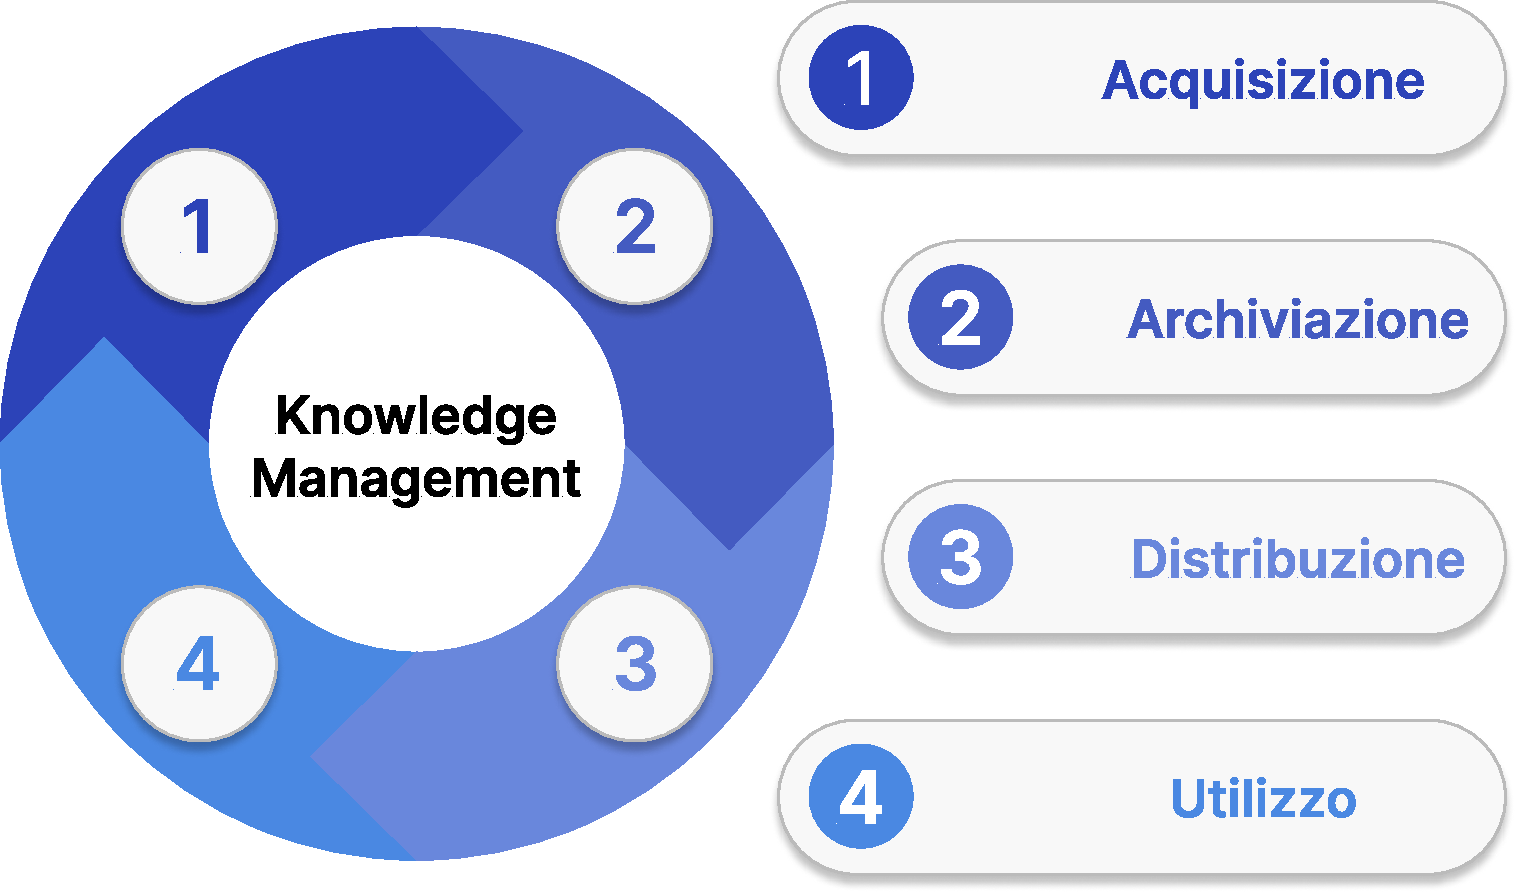
\includegraphics[width=0.8\linewidth]{figure//capitolo_3/Knowledge Management Process.pdf}
    \caption{Ciclo dell'informazione}
    \label{fig:Knowledge Management Process}
\end{figure}

\subsection{Sistemi per la Gestione della Conoscenza}

Prima dell'avvento della tecnologia, la gestione della conoscenza avveniva attraverso canali di comunicazione analogici e la conservazione di tale conoscenza era lasciata alle biblioteche. Tuttavia, con l'evoluzione della scienza è stato possibile per l'uomo di disporre di strumenti tecnologici che potessero semplificare tale compito, comportando cambiamenti non solo nel sistema di archiviazione ma anche nelle metodologie da applicare per svolgerlo. A questo scopo sono nati degli applicativi che permettessero di supportare le fasi del ciclo dell'informazione e della sua gestione.

Più precisamente, un \textbf{sistema di gestione della conoscenza} (\textit{Knowledge Management System, KMS}) sfrutta la conoscenza collettiva dell'azienda per portare migliori efficienze operative. Tali sistemi sono supportati dall'utilizzo di una conoscenza di base. Di solito sono fondamentali per una gestione efficiente ed efficace della conoscenza in questione, creando un ambiente centralizzato per memorizzare le informazioni e accedervi velocemente secondo le necessità del caso \cite{ibm_knowledge_management}.

\subsection{Scoperta della Conoscenza nei Database (Knowledge Discovery in Databases)}

A livello astratto, il campo della \textbf{Knowledge Discovery in Databases} (\textit{KDD}) si occupa dello sviluppo di metodi e tecniche per dare senso ai dati. Il problema di base affrontato dal processo KDD consiste nel mappare dati a basso livello (che sono tipicamente troppo voluminosi per essere compresi e assimilati facilmente) in altre forme che potrebbero essere più compatte, più astratte o più utili. Al centro del processo c'è l'applicazione di specifici metodi di data mining per la scoperta e l'estrazione di pattern \cite{from_data_mining_to_knowledge_discovery}.

La frase “knowledge discovery in databases” viene attribuita al data scientist Usama Fayyad a seguito di un workshop tenuto nel 1989, dove venne usata per esplicitare che il risultato finale dell'indagine sui dati dovrebbe essere la scoperta di conoscenze utilizzabili. La KDD comprende tutti i processi, automatizzati e non, che migliorano o consentono l'esplorazione di database (indipendentemente dalle loro dimensioni), per recuperare potenziali conoscenze \cite{knowledge_discovery_in_databases}.

\subsubsection{Il Processo KDD}

Il processo KDD è di tipo iterativo e interattivo (dove molte delle decisioni sono dipendenti dalle scelte dell'utente) e coinvolge nove differenti fasi \cite{researchgate_data_mining_and_knowledge}, ovvero:

\begin{enumerate}
    \item \textit{Apprendimento del dominio dell'applicazione}. Questa fase comprende lo sviluppo della comprensione delle conoscenze pregresse pertinenti e degli obiettivi dell'applicazione.
    \item \textit{Creazione di un set di dati target}. Questa fase include la selezione di un set di dati o la focalizzazione su un sottoinsieme di dati su cui bisogna effettuare la scoperta della conoscenza.
    \item \textit{Pulizia e pre-elaborazione dei dati}. Questa fase svolge le operazioni di base per la pulizia dei dati, la raccolta di informazioni utili alla modellazione, la definizione di regole per la gestione dei campi mancanti e la gestione del database.
    \item \textit{Riduzione e proiezione dei dati}. Questa fase comprende la ricerca di caratteristiche utili per rappresentare i dati e l'uso di metodi per la diminuzione delle dimensioni o del numero di variabili da prendere in considerazione.
    \item \textit{Scelta della funzione di data mining}. Questa fase si occupa di decidere lo scopo del modello derivato dall'applicazione dell'algoritmo di data mining.
    Scelta dell'algoritmo di data mining. Questa fase include la selezione dei metodi da adoperare per cercare modelli nei dati.
    \item \textit{Data mining}. Questa fase effettua la ricerca dei modelli di interesse in una particolare forma di rappresentazione o in un insieme di tali rappresentazioni.
    \item \textit{Interpretazione dei modelli}. Questa fase comprende l'interpretazione dei modelli scoperti dalla fase precedente e, se necessario, la riapplicazione di alcune delle fasi già svolte.
    \item \textit{Utilizzo della conoscenza scoperta}. Questa fase include l'integrazione della conoscenza appresa nel sistema di performance, intraprendendo azioni basate s tale conoscenza o semplicemente documentarla.
\end{enumerate}

In generale è possibile raggruppare queste fasi in cinque passaggi essenziali che permettono di descrivere a pieno il processo KDD \cite{knowledge_science}, ovvero:

\begin{enumerate}
    \item \textit{Comprendere il dominio dell'applicazione per formulare il problema}. Questo è chiaramente il prerequisito per recuperare informazioni utili e scegliere dei metodi appropriati di apprendimento automatico ed estrazione dati, dipendentemente dallo scopo finale dell'applicazione e dalla natura dei dati di origine.
    \item \textit{Raccolta e pre-elaborazione dei dati}. Questo passaggio comprende la selezione delle fonti dati, la rimozione di eventuali rumori e anomalie, la gestione di eventuali dati mancanti, la trasformazione e la riduzione del volume di dati. Date queste numerose operazioni, questo è il passaggio che richiede maggior tempo nell'intero processo.
    \item \textit{Data mining}. Questo passaggio è necessario per l'estrazione dei modelli o pattern nascosti dei dati.
    \item \textit{Interpretazione (o post-elaborazione) dei dati}. Questo passaggio si occupa di interpretare la conoscenza scoperta mediante l'uso dei metodi di natura induttiva. Gli esperimenti mostrano che i pattern o i modelli scoperti dai dati non sono sempre di interesse o utilizzo diretto, e il processo di KDD è necessariamente iterativo con la valutazione della conoscenza scoperta.
    \item \textit{Applicazione delle conoscenze}. In alcuni casi, non è necessario adoperare sistemi informativi per sfruttare la conoscenza scoperta, mentre in altri casi l'utente può aspettarsi che questa possa essere inserita nei propri dispositivi di analisi per essere messa a disposizione di diversi programmi.
\end{enumerate}

\begin{figure}[!h]
    \centering
    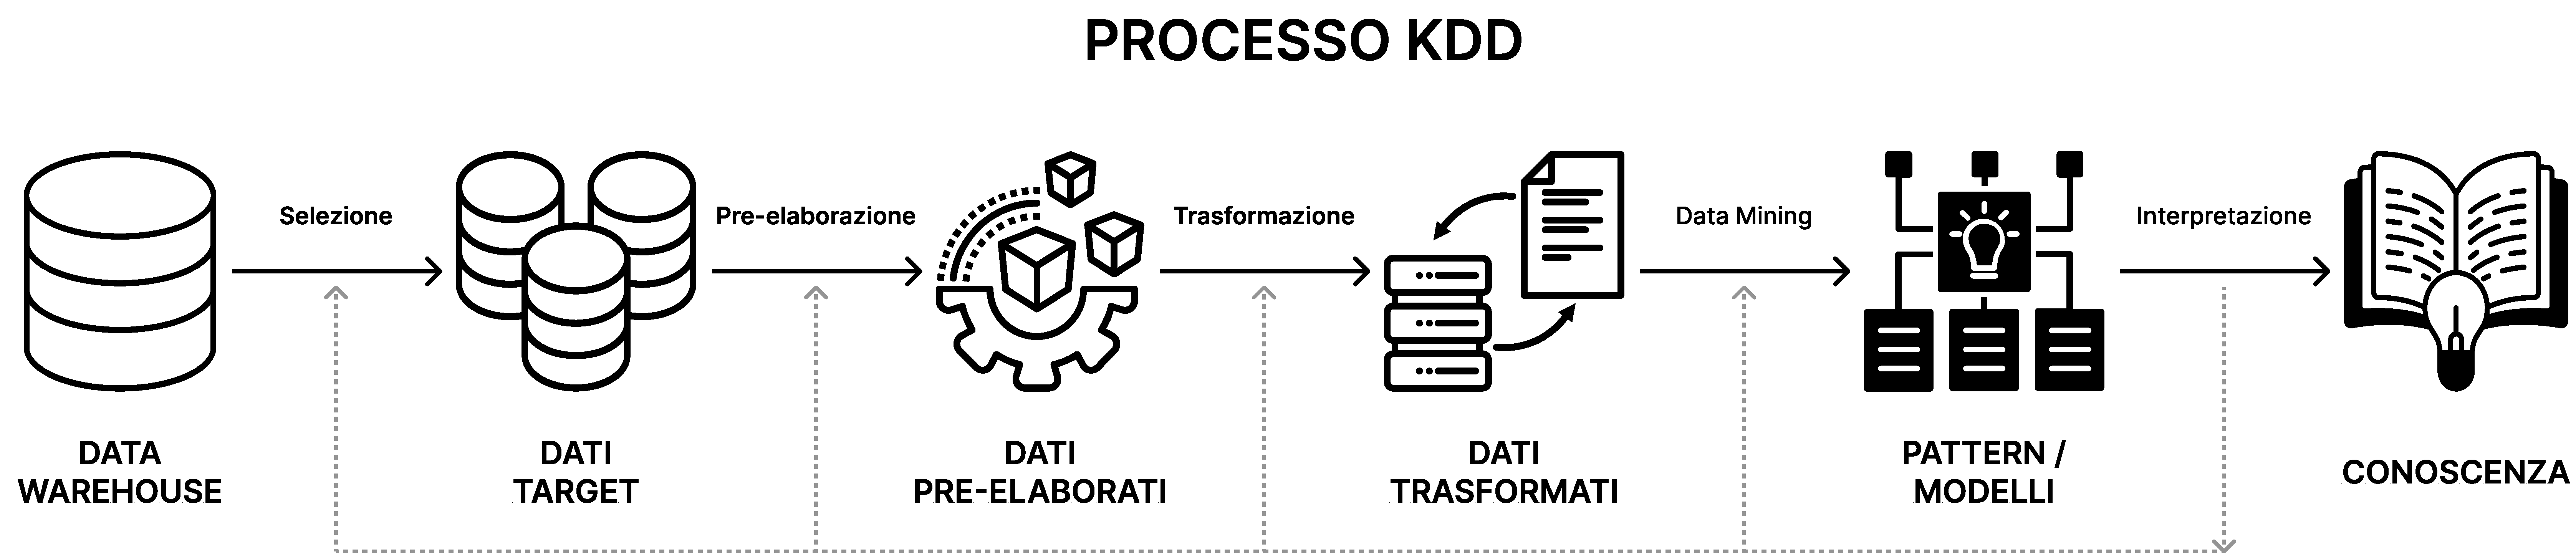
\includegraphics[width=1\linewidth]{figure//capitolo_3/KDD Process.pdf}
    \caption{Processo KDD}
    \label{fig:KDD Process}
\end{figure}

\subsection{Data Mining}

Il \textbf{Data Mining} (\textit{DM}) è la fase di estrazione della conoscenza, essenziale in un processo di KDD, da una grande quantità di dati oppure un data warehouse. Per effettuare questa estrazione, il data mining combina l'intelligenza artificiale, l'analisi statistica e i DBMS nel tentativo di estrarre conoscenze dai dati archiviati. Più semplicemente, è possibile dire che il DM è il processo di applicazione di specifici metodi per estrarre dei \textit{pattern} o \textit{modelli} dai dati \cite{citeseerx_data_mining}.

Secondo Fayyad, il Data Mining svolge sei principali funzioni \cite{aircconline_data_mining}:

\begin{enumerate}
    \item \textit{Classificazione}: consiste nel trovare modelli che analizzano e classificano uno specifico dato in diverse classi predefinite.
    \item \textit{Regressione}: consiste nell'associare uno specifico dato ad una variabile di previsione con valori reali.
    \item \textit{Clustering}: consiste nell'identificare un insieme finito di categorie o cluster per descrivere i dati.
    \item \textit{Modellazione delle dipendenze} (comprensione delle regole di associazione): consiste nel trovare un modello che descriva dipendenze significative tra le variabili.
    \item \textit{Rilevamento delle deviazioni} (rilevamento delle anomalie): consiste nello scoprire i cambiamenti più significativi nei dati.
    \item \textit{Riepilogo}: consiste nel trovare una descrizione compatta per un sottoinsieme specifico di dati.
\end{enumerate}

\subsubsection{Differenza tra Data Mining e KDD}

Data questa introduzione è possibile comprendere come il termine “Data Mining” è improprio rispetto al processo che ha l'obiettivo, non di estrarre direttamente i dati, bensì sfruttare gli archivi di dati, laddove ne sia presente una grande quantità, per estrarne il significato o ricavarne una conoscenza da questi che possa essere definita preziosa \cite{aws_data_mining}.

Dato che molto spesso si fa confusione con i termini e le definizioni di \textit{scoperta della conoscenza dei database} e \textit{data mining}, di seguito è riportata una tabella riassuntiva che permette di capirne le differenze \cite{geeksforgeeks_data_mining}:

\begin{comment}
\begin{table}[!h]
    \centering
    \begin{tabular}{ccc}
        Parametro & KDD & DM\\
        Definizione & Processo di identificazione di modelli e relazioni validi, nuovi, potenzialmente utili e comprensibili nei dati. & Processo di estrazione di informazioni o modelli utili e preziosi da set di dati di grandi dimensioni.\\
        Obiettivo & Trovare conoscenza utile dai dati. & Per estrarre informazioni utili dai dati.\\
        Tecniche adoperate & Pulizia, integrazione, selezione, trasformazione dei dati, data mining, valutazione dei modelli e rappresentazione e visualizzazione della conoscenza. & Regole di associazione, classificazione, clustering, regressione, alberi decisionali, reti neurali e riduzione delle dimensioni dei dati.\\
        Output & Informazioni strutturate, come regole e modelli, che possono essere utilizzate per prendere decisioni o previsioni. & Modelli, associazioni o intuizioni che possono essere utilizzati per migliorare il processo decisionale o la comprensione.\\
    \end{tabular}
    \caption{Differenze tra il processo KDD ed il Data Mining}
    \label{tab:kdd_vs_data_mining}
\end{table}
\end{comment}